\section{May 2022}

\subsection*{Classical Mechanics}
\addcontentsline{toc}{subsection}{Classical Mechanics}

\prob{1.1}{

Two (1-dimensional) pendula made of massless rods of equal length $L$ and points of masses $m$ and $M$ at the end are hung side-by-side.
The ends of pendula are connected by a spring constant $k$ that is in its relaxed state when both pendula hang straight down.

\begin{parts}
    \item Using the two angles $\phi_1$ and $\phi_2$ of the two rods with the vertical as generalized coordinates, and the small-angle approximation, write down the Lagrangian for this problem.

    \item Recast the Lagrangian into the form
    \begin{align*}
        \frac{1}{2} \dot{\vec{\phi}} \vb*{T} \dot{\vec{\phi}} - \frac{1}{2} \vec{\phi} \vb*{V} \vec{\phi}
    \end{align*}
    with $2 \times 2$ matrices $\vb*{T}$ and $\vb*{V}$.

    \item Write down the Euler-Lagrange equations in the same matrix form, and insert the ansatz
    \begin{align*}
        \vec{\phi}(t) = \vec{a} \exp( -i \omega t )
    \end{align*}
    to end up with an ``eigenvalue'' equation for $\lambda = \omega^2$.

    \item Find the possible values for $\lambda_{1,2}$ and the corresponding fundamental modes $\vec{a}_{1,2}$ (No need to normalize them).

    \item Describe and contrast the two fundamental modes: What does the motino look like in each case, and what frequency does it have?
\end{parts}

}

\sol{}


\prob{1.2}{

There is a cylinder with radius $a$ and mass $m$ rolling without slipping on top of another, fixed cylinder with radius $b$.
The first cylinder starts out exactly on top of the second cylinder. (See the figure below.) Write down the equations of motion for the time period \textit{before} the top cylinder disconnects from the bottom cylinder.
Express your answer in terms of $\theta$ and its derivatives, $r = a + b$, $b$, and $m$.

\begin{center}
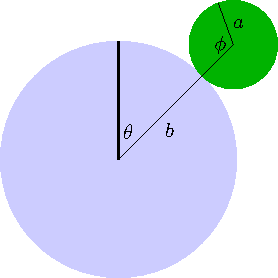
\includegraphics{May2022/1-2.pdf}
\end{center}

}

\sol{}


\prob{1.3}{

A particle of mass $M$ is attached by a massless rod of length $a$ to a small ring of mass $m$, free to slide on a fixed horizontal bar.
The string moves in the vertical plane through the bar.

\begin{center}
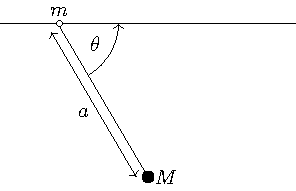
\includegraphics{May2022/1-3.pdf}
\end{center}

\begin{parts}
    \item Write down the Lagrangian and Euler-Lagrange equations for the system.

    \item Find conserved quantities.

    \item Find frequency of small oscillations, if any.
\end{parts}

}

\sol{}


\prob{1.4}{

Two bodies move under the influence of the potential $V(r) = k r^{\alpha}$ where $\vb*{r}$ is the relative coordinate and $k$ and $\alpha$ are constants.

\begin{parts}
    \item If $\vb*{r} = \vb*{f}(t)$ is a solution of the equation of motion, show that $\vb*{r} = \lambda \vb*{f}(\lambda^{\sigma} t)$ is also a solution for any $\lambda$ provided $\sigma$ is suitably chosen.

    \item Apply the result of part (a) to the cases $\alpha = 2$ (harmonic oscillator) and $\alpha = -1$ (Kepler problem).
    Comment on the results and on the properties you can derive from them.
\end{parts}

\textbf{Hint}: Use $m \ddot{\vb*{r}} = - \nabla V(\vb*{r})$.

}

\sol{}


\prob{2.1}{

Find the minimal distance between two particles when one of them (having mass $m$) moves from infinity with velocity $v$ and impact parameter $\rho$ towards the second one that is initially at rest (and has mass $M$).
The potential energy of the particle's interaction is given by $U(r) = -U_0 (R/r)^2$, where $r$ is the distance between particles, while $U_0 > 0$ and $R$ are constants.

}

\sol{}

\subsection*{Electricity \& Magnetism}
\addcontentsline{toc}{subsection}{Electricity \& Magnetism}

\prob{2.2}{

Consider an infinitely long straight wire along the $z$-axis.
Suppose the wire gets a sudden current by $I(t) = a \delta(t)$, where $a$ is a constant and $\delta(t)$ is the Dirac delta function.
Find

\begin{parts}
    \item the electric and magnetic potentials $\Phi(\vb*{r},t)$, $\vb*{A}(\vb*{r},t)$, and

    \item electric and magnetic fields $\vb*{E}(\vb*{r},t)$, $\vb*{B}(\vb*{r},t)$
\end{parts}

}

\sol{}


\prob{2.3}{

Two thin coaxial rings, each of radius $a$, are a distance $b$ apart, and each uniformly charged with charges $Q_1$ and $Q_2$.
The work required to bring a point charge $q$ from infinity up to the centers of each of the two rings is $W_1$ and $W_2$, respectively.
Show that the charges on the rings are
\begin{align*}
    Q_{1,2} = \frac{4 \pi \epsilon_0 a}{b^2 q} ( a^2 + b^2 )^{1/2} \Big[ (a^2 + b^2)^{1/2} W_{1,2} - a W_{2,1} \Big]
\end{align*}

}

\sol{}


\prob{2.4}{

The region bounded by two concentric spherical surfaces is filled with a uniform charge density $\rho_0$ (constant).
On the inner boundary ($r = a$) of this region, the potential is
\begin{align*}
    \Phi(a,\theta) = V_0 \cos{\theta}
.\end{align*}
On the outer boundary ($r = b$) of this region, the potential is
\begin{align*}
    \Phi(b,\theta) = 2 V_0
.\end{align*}
Find the solution of Poisson's equation in the region $a \leq r \leq b$.

}

\sol{}


\prob{3.1}{

The $\phi$ particle, which is a bound state $\bar{s}s$ of strange quarks, has mass approximately equal to $1.02~{\rm GeV}/c^2$.

\begin{parts}
    \item What is the minimal (``threshold'') energy of electrons necessary to produce $\phi$ particles in the reaction $ep \rightarrow ep\phi$ at JLab electron accelerator?

    \item What is the velocity and energy (in laboratory frame) of $\phi$ particles produced at threshold?
\end{parts}

}

\sol{}


\prob{3.2}{

An infinitely long, nonconducting solid cylinder of radius $R$ has a \textbf{nonuniform volume charge density} $\rho(r)$ that is a function of the radial distance $r$ from the axis.
See the diagram below.
Say that this charge density is $\rho(r) = B r^2$, where $B$ is a constant with units of $\mu{\rm C}/m^5$.
Use Gauss' law to find the magnitude $E$ of the resulting electric field when

\begin{parts}
    \item $0 < r < R$, and

    \item $r > R$.
\end{parts}

Express your answers in terms of $B$, $r$, $R$, and any constants.

\begin{center}
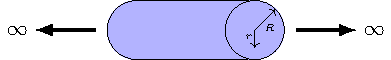
\includegraphics{May2022/3-2.pdf}
\end{center}

}

\sol{}


\prob{3.3}{

A plane electromagnetic wave with frequency $\omega$ traveling in vacuum along the $z$-axis (from $-\infty$) is given by
\begin{align*}
    \vb*{E}_{\rm in}(\vb*{r},t) &= E_{0 ,\rm in} \vu*{x} \exp[i(kz - \omega t)] \\
    \vb*{B}_{\rm in}(\vb*{r},t) &= E_{0,\rm in} \vu*{x} \exp[i(kz - \omega t)]
,\end{align*}
where $k = \omega/c$ and $c$ is the speed of light (Gaussian units).
At $z = 0$, the wave encounters an interface with a semi-infinite, linear dielectric medium filling the entire half-space $z > 0$.
This medium has a dielectric constant (relative electric permittivity) $\epsilon > 1$ but unit magnetic permeability $\mu = 1$ and hence $\vb*{B} = \vb*{H}$.
As a consequence, the medium has an index of refraction $n = \sqrt{\epsilon} > 1$ and a propagation speed $c / n < c$.
Therefore, the transmitted part of the electromagnetic wave in the medium has an electric field given by
\begin{align*}
    \vb*{E}_{\rm tr}(\vb*{r},t) &= E_{0 ,\rm tr} \vu*{x} \exp[i(nkz - \omega t)]
.\end{align*}
Finally, because of the boundary conditions (see below), there must also be a reflected wave going in the negative $z$-direction, with electric field
\begin{align*}
    \vb*{E}_{\rm re}(\vb*{r},t) &= E_{0 ,\rm re} \vu*{x} \exp[-i(kz + \omega t)] \\
\end{align*}

\begin{parts}
    \item Determine the amplitudes $B_{0,\rm tr}$ and $B_{0,\rm re}$ of the magnetic fields of the transmitted and reflected waves,
    \begin{align*}
        \vb*{B}_{\rm tr}(\vb*{r},t) &= B_{tr} \vu*{x} \exp[i(nkz - \omega t)] \\
        \vb*{B}_{\rm re}(\vb*{r},t) &= B_{0 ,\rm re} \vu*{x} \exp[-i(kz + \omega t)] \\
    \end{align*}
    in terms of the corresponding amplitudes $E_{0,\rm tr}$ and $E_{0,\rm re}$. (It is best to use the last of Maxwell's equations, $\nabla \times \vb*{E} + \frac{1}{c} \frac{\partial \vb*{B}}{\partial t} = 0$.)

    \item Using the requirement that \textbf{both} the sum of all electric fields and the sum of all magnetic fields must be continuous at $z = 0$ (why?), determine the relative size of the amplitudes $E_{0,\rm tr}$ and $E_{0,\rm re}$ in terms of $E_{0,\rm in}$.

    \item Calculate the amplitude of the Poynting vector, $\vb*{S}_0 = \frac{c}{4\pi} \vb*{E}_0 \times \vb*{B}_0$, for all three waves, and show that energy is conserved (\textit{i.e.} as much energy is carried in by the incoming wave per unit time as the reflected and transmitted waves carry out).
\end{parts}

}

\sol{}

\subsection*{Quantum Mechanics}
\addcontentsline{toc}{subsection}{Quantum Mechanics}

\prob{3.4}{

A particle of mass $m$ is trapped by a very thin spherical shell of radius $R$ modeled by the potential $U(r) = -V \delta(r - R)$ with $V > 0$.
Consider only the s-state with zero orbital momentum and obtain:

\begin{parts}
    \item The equation for the ground state energy of the bound state.

    \item The critical radius $R_c$ below which the bound state in the well disappears.
\end{parts}

}

\sol{}

\prob{4.1}{

An electron is at a fixed position in an oscillating magnetic field
\begin{align*}
    \vb*{B}(t) = B_0 \cos(\omega t) \vu*{z}
,\end{align*}
wherer $B_0$ and $\omega$ are constants.

\begin{parts}
    \item Write down the Hamiltonian for this system.

    \item The electron is at time $t = 0$ in the spin state with eigenvalue $\hbar/2$ with respect to the $x$-axis.
    Determine the spin state of the electron at later times.

    \item Obtain the probability of obtaining $-\hbar/2$ if one measures $S_x$.
\end{parts}

}

\sol{}


\prob{4.2}{

Define a coherent state
\begin{align*}
    \ket{\alpha} = \exp( -\frac{|\alpha|^2}{2} ) \sum_{n=0}^{\infty} \frac{\alpha^n}{\sqrt{n!}} \ket{n}
,\end{align*}
where $\alpha$ is an arbitrary complex number and $\ket{n}$ is the eigenstate of the harmonic oscillator of energy $\hbar \omega (n + 1/2)$.

\begin{parts}
    \item Show that $\bra{\alpha}\ket{\alpha} = 1$ and $\ket{\alpha} = \exp(-|\alpha|^2/2) \exp(\alpha a^{\dagger}) \ket{0}$.

    \item Show that coherent states are eigenstates of the annihilation operator $a \ket{\alpha} = \alpha \ket{\alpha}$.
\end{parts}

}

\sol{}


\prob{4.3}{

Consider a particle of charge $q$ and mass $m$ in one dimension in a harmonic oscillator potential and under the influence of a uniform electric field.
The Hamiltonian reads
\begin{align*}
    \hat{H} = \hat{H}_0 + \hat{V}, \quad \hat{H}_0 = \frac{\hat{p}^2}{2m} + \frac{m \omega^2}{2} \hat{x}^2, \quad \hat{V} = -q E \hat{x}
.\end{align*}
Assume that the electric field is weak, so that a perturbative calculation is permissible.
The eigenenergies and eigenstates of the harmonic oscillator are well known:
\begin{align*}
    \hat{H}_0 \ket{n} = \hbar \omega (n + 1/2) \ket{n} = \epsilon_{n} \ket{n}
.\end{align*}

\begin{parts}
    \item Calculate the correction (up to including second order) to a generic energy level.

    \item Obtain the exact eigenenergies of $\hat{H}$ and compare them with the results obtained in part (a) above.

    \item Without doing any detailed calculation, explain why the third order correction to a generic level vanishes.
\end{parts}

\textbf{Hint}: Note that, if the first-order correction $E_n^{(1)}$ vanishes, then the third-order correction to a non-degenerate energy level due to a perturbation $\hat{V}$ is simply given by
\begin{align*}
    E_n^{(3)} = \sum_{a,b \ne n} \frac{V_{na} V_{ab} V_{bn}}{(\epsilon_a - \epsilon_n)(\epsilon_b - \epsilon_n)}
.\end{align*}

}

\sol{}


\prob{4.4}{

Two nonidentical spin-1/2 particles interact via the Hamiltonian
\begin{align*}
    \hat{H} = A( \sigma_z^{(1)} + \sigma_z^{(2)} ) + B \vb*{\sigma}^{1} \cdot \vb*{\sigma}^{(2)}
,\end{align*}
where $\sigma_x$, $\sigma_y$, and $\sigma_z$ are the Pauli $\sigma$-matrices and $\vb*{\sigma} = (\sigma_x,\sigma_y,\sigma_z)$.
The ``(1)'' and ``(2)'' superscripts label particles 1 and 2 respectively.
$A$ and $B$ are real constants.

Find the energy eigenvalues.

\textbf{Hint}: Notice that you can classify the states in terms of the eigenstates of the total spin operators $\hat{S}_z = \frac{\hbar}{2}( \sigma_z^{(1)} + \sigma_z^{(2)} )$ and $\hat{S}^2 = \frac{\hbar^2}{4}( \vb*{\sigma}^{(1)} + \vb*{\sigma}^{(2)} )^2$ since they commute with $\hat{H}$.

}

\sol{}
